\documentclass[11pt,a4paper,titlepage]{report}


% Document settings

\title{OSP Project Specification \\ Team $\langle$sql injection$\rangle$}

\author{
  Neil Ang\\
  \texttt{s3251533}
  \and
  ``Alfred" Yang Yuan\\
  \texttt{s3363619}
  \and
  Val Lyashov\\
  \texttt{s3366222}
}

\date{Semester 2, 2013}


% Change section numbering
%\renewcommand\thesection{\Roman{section}}
%\renewcommand\thesubsection{\Alph{subsection}}
\renewcommand\thesection{\arabic{section}}
\renewcommand\thesubsection{\thesection.\arabic{subsection}}


% Enable smart quotes
\usepackage [english]{babel}
\usepackage [autostyle]{csquotes}
\MakeOuterQuote{"}


% Set watermark while in development
\usepackage{draftwatermark}
\SetWatermarkText{DRAFT}
\SetWatermarkScale{5}
\SetWatermarkColor[gray]{0.95}


% Alias pi name
\usepackage{xspace}
\newcommand{\rpi}{\textit{Raspberry Pi\textsuperscript{\textregistered}}}
\newcommand{\rpis}{\textit{Raspberry Pi\textsuperscript{\textregistered}s}}

% Side by side graphics
\usepackage{graphicx}
\usepackage{caption}
\usepackage{subcaption}

% Switch to biblatex
\usepackage{biblatex}
\bibliography{computer-vision}
\bibliography{audio}
\bibliography{servo}

% Add the bib to the toc
\DefineBibliographyStrings{english}{
  bibliography = {Bibliography},
}

%For process listing
\usepackage{dirtree}
%\usepackage{qtree}

\usepackage{multicol}

% Stop tables being repositioned
\usepackage{float}
\restylefloat{table}

% Better table height
\usepackage{tabu}

% The appendix
\usepackage{appendix}

% Code highlighting
\usepackage{listings}
\lstset{basicstyle=\ttfamily}

% For marking what's left to do
\usepackage{color}


\begin{document}


\maketitle

\pagebreak
\tableofcontents
\thispagestyle{empty}
\pagebreak

\section{Introduction}

Our project will attempt to modernise the phonograph, by using the \rpi\xspace for subject tracking, digital recording and audio processing. A directional microphone will installed on a custom mount that can be programmatically moved in an X and Y direction. An additional camera will be used to detect the subject (e.g. a human face), and adjust the position of the microphone accordingly. The secondary of task of the project is to process the audio recordings through an Internet based voice-to-text service.

The final solution will be a relatively cheap, portable and smart recording device suitable for use in a lecture theatre or classroom. It would be ideal for assisting students in note taking, or for lecturers teaching in learning spaces that haven't been outfitted with full featured recording systems (such as the \textit{Lectopia}\footnote{http://www.rmit.edu.au/teaching/technology/lecturecapture} or \textit{Echo360}\footnote{http://www.rmit.edu.au/teaching/technology/echo360} systems used at \textit{RMIT}).


\section{System Overview}

This is an ambitious project and involves a lot of complex processing and interaction with hardware. To distribute the CPU workload and modularise the solution, the functionality will be spread over two \rpis. This will also have the added benefit of making it easier to work on as a group, because the parts can be developed independently of each other.

\begin{figure}
\centering
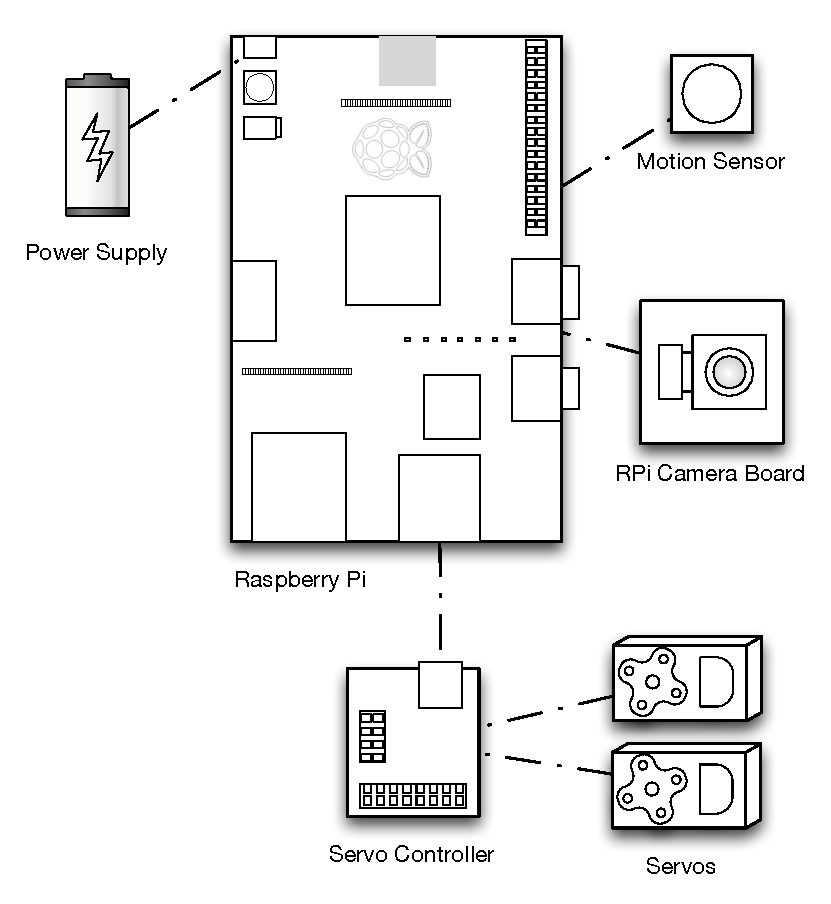
\includegraphics[width=0.6\textwidth]{graphs/rpi_1.pdf}
\caption{Connected hardware for computer vision component of project. It includes a power supply, motion sensor, RPi camera board, servo controller and two servos.}
\label{fig:cvhardware}
\end{figure}


The first \rpi\xspace will be responsible for subject tracking via computer vision. It will detect the subject via an attached camera and communicate directly with a servo controller to move the microphone mount. In an effort to conserve power, this \rpi\xspace will also have a motion sensor connected to one of its General Purpose Input/Output (GPIO) ports. When no motion is detected, it will power down the connected peripherals. Figure \ref{fig:cvhardware} illustrates the connected components for this device.


\begin{figure}
\centering
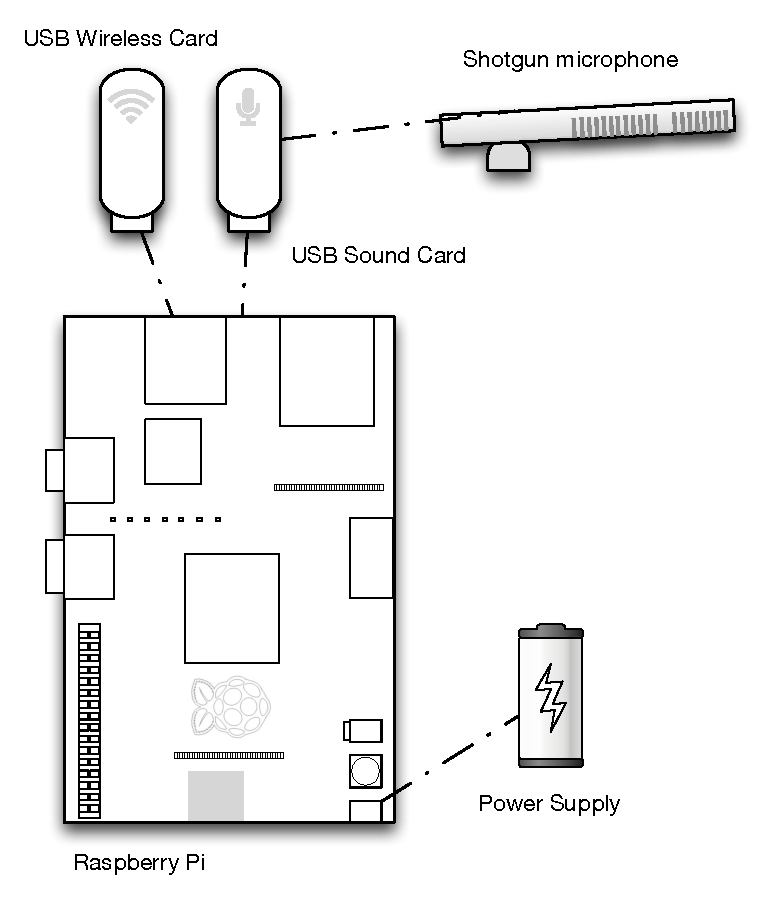
\includegraphics[width=0.6\textwidth]{graphs/rpi_2.pdf}
\caption{Connected hardware for audio recording component of project. It includes a power supply, sound card, shotgun microphone and wireless card.}
\label{fig:audiohardware}
\end{figure}

The second \rpi\xspace will be responsible for the audio recording and processing. It will be connected to a shotgun microphone attached for direction recording with minimal noise interference. An addition USB sound card will also included to support the recording. The intention is to also perform voice-to-text processing through a web service, so a wireless card will also be attached for communication with the Interned. Figure \ref{fig:audiohardware} illustrates the connected components for this device.

Both \rpis\xspace will be networked together via the Ethernet ports for inter-device communication.

For a detailed summary of all involved hardware and its purpose in the project, see Table \ref{table:hardwaretable}. 


\begin{center}
\begin{table}
{\tabulinesep=2mm
\begin{tabu}{ lcp{7cm} }

    \textbf{Hardware} & \textbf{Qty} & \textbf{Purpose} \\ \hline
    
    \rpi & 2 & Due to the inherent complexity of audio and video processing, the solution workload will be split across two \rpis. The first will handle the computer vision and controlling the servos. The second is for processing audio and data storage.\\ 

    \textit{Camera} & 1 & Either a RPi Camera board or USB web cam will be used for subject tracking through computer vision. \\ 
    
   \textit{Servos} & 2 & Two servos will be used to control the microphone mount. One servo will manoeuvre the mount on an X axis, while the other is used for the Y axis. \\ 
        
    \textit{USB servo controller} & 1 & This will be used to improve the movement accuracy of the servos \\ 
    
    \textit{USB sound card} & 1 & The \rpi\xspace has no in-built audio input jack, so an external sound card will be used to facilitate connecting the microphone. \\ 
    
    \textit{Shotgun microphone} & 1 & This microphone will give us targeted audio for recording voice and minimising background noise. \\ 
    
    \textit{Motion sensor} & 1 & To conserve battery before and after a recording session, a low-power motion sensor will be used to detect the presence of a subject in the room. The solution will return to "standby mode" if no movement is detected.\\ 

    \textit{Power supply} & 2 & To take advantage of the lightweight nature of the \rpi\xspace and components, an external battery pack will be used to make the solution portable.\\ 


    \textit{Wireless card} & 1 & The voice-to-text processing will be performed remotely, so an unobtrusive internet connection will be required.\\ \hline
    
\end{tabu} }
\caption{Summary of hardware}
\label{table:hardwaretable}
\end{table}

\end{center}

\section{Design Considerations}

We want the system to run efficiently, but early experiments have suggested that the face detection will be very CPU intensive. We've decided that Python is acceptable for prototyping components, but for optimal performance we will need to port all our software to C and C++ implementations.

Another one of our goals is to design this as a portable solution. For this to occur we will need to factor in power consumption. Powering the solution by battery is not difficult, but we will need to intelligently invent ways to reduce resource usage to increase battery performance. This will include powering hardware on and off when not in use and reducing CPU usage to a minimum. Although we will endeavour to design the project to be power conservative, we will only explore  battery power if we have time remaining at the end of the project. 

{\color{red} Storage capability for prolonged usage. Modularity of components. }


\subsection{Goals and Objectives}

This project aims to provide an easy way to audio record and annotate lectures, talks and other presentations. However we are also attempting to meet all learning objectives of the assignment as well.

\begin{description}
   
  \item[Personal goals] \hfill \\
      Design a solution that is to be relatively portable, requires minimal setup and start-up time. 
      
  \item[Learning objective 1] \hfill \\
%\textit{Design, develop, test, and debug a complex system-level program on a resource constrained device using appropriate development environments, debuggers, unit testing tools, and version control tools.}
%\\ \\
  {\color{red} TODO: Add info about the design and develop environment.}

The \rpi\xspace is a resource constrained device, so our objective is to ensure that our system runs efficiently with the hardware available. We will achieve this by running performance tests for all software components and introducing clever ways (e.g. using the motion sensor) to reduce CPU and conserve power. {\color{red} TODO: add the debugger we will use.}

All source code and project documentation for this project is version controlled through \textit{git}, and hosted on a private\footnote{Access to this repository is available upon request.} \textit{GitHub} repository along with our project wiki and development logs.

  \item[Learning objective 2] \hfill \\
%\textit{Assess how computing resources are used by the application software and managed by the system software. Analyse the inherent trade-offs between hardware constraints and system software.}
%\\ \\
The system will be built on a bare-bones linux distribution and designed so that each sub-components of the main software application will take responsibility for interfacing with only one hardware feature (e.g. the \textit{comms} will be the only process that can access the ethernet port, and the \textit{face-detect} process will be the only one that can access the camera). Building the solution this way, with no other programs competing for resources is how we will effectively manage the hardware.

{\color{red} TODO: how will we analyse the trade offs between hardware/software?}


  \item[Learning objective 3] \hfill \\
  %\textit{Construct appropriate diagrams and textual descriptions to communicate a system level program design and how it integrates one or more of the following key OS concepts: a. kernel and hardware interaction; b. processes and interprocess communication; c. concurrency and synchronisation; d. pre-emptive and non-preemptive scheduling; e. memory hierarchy, management, and cost-performance trade-offs; f. file system design and implementation; and/or g. security and privacy.}
%// // 
This will be covered in the final portfolio through diagrams of the system design.

  \item[Learning objective 4] \hfill \\
%\textit{Describe the full range of considerations of effective and efficient teamwork.}
The team has been given primary roles which make use of their best skills. However, to increase each group members personal learning in areas they are not already accomplished in, we've allowed for some overlap in the roles. For example, Val who has expertise in Unix/Hardware, will also attempt to prototype some of the hardware interfaces in Python. Neil, who doesn't have much hardware or C++ experience, will then port the Python scripts to C++. The primary responsibilities for the roles will still lie with designated group member, but everyone will have the opportunity to try something they haven't done before.

\end{description}




\subsection{Assumptions and Dependencies}

{\color{red} We are dependant on the OpenCV library...}

\subsection{General Constraints}

A major constraint of this project it the processing power of the \rpi. Preliminary investigations suggest that depth sensing would be a more accurate subject tracking technique, but the \rpi\xspace would not have the processing power required for skeletal mapping. Therefore we have opted to do face detection, but its effectiveness will be limited by the light in the room, the direction the subject is facing and any obstruction of the facial features.

As we are building moving parts into the project, we will also be constrained by the total weight of the hardware. There is a physical limit the servos torque and we have to ensure our mount is designed so it doesn't exceed it.

However the biggest constraint of the project is time. The project is very ambitious, with a lot of things that could not turn out as originally planned. Adapting to these situations will become increasingly limiting as we approach the delivery date.


\subsection{Development Methodology}

The project will constructed over 3 main stages in isolated parts by all group members. 


\subsubsection{Stage 1}

The first stage will attempt to solve the hardest issues of face recognition and physical movement. We will also need to demo our cross-compiler and develop the project specification.

\begin{table}[H]
\begin{tabular}{|l|c|c|}
    \hline
    \textbf{Objective} & \textbf{Members} & \textbf{Week} \\ \hline
    
    Lab demo & All & 5 \\ \hline
    OpenCV tracking & Alfred, Neil & 4, 5, 6 \\ \hline
    Servo movement & Val & 4, 5, 6 \\ \hline
    Project Specification & Neil & 6 \\ \hline

\end{tabular}
\end{table}

\subsubsection{Stage 2}

Stage two will also encapsulate the mid-semester break. We will combine what was built in the first stage and start work on implementing the features of the second \rpi.

\begin{center}
\begin{table}[H]
\begin{tabular}{|l|c|c|}
    \hline
    \textbf{Objective} & \textbf{Members} & \textbf{Week} \\ \hline
    
    Servo Mount & Val & 7 \\ \hline
    Audio recording & Val & 8 \\ \hline
    Pi device comms & Alfred & 7 \\ \hline
    Server complete & Alfred & 8 \\ \hline
    PIR monitor & Neil & 7 \\ \hline
    Integrated Face tracking /w Servo & Neil & 8 \\ \hline


\end{tabular}
\end{table}
\end{center}


\subsubsection{Stage 3}

Final stage will involve putting all the finished pieces together. We will also need to deliver our presentation and portfolio in this stage.


\begin{center}
\begin{table}[H]
\begin{tabular}{|l|c|c|}
    \hline
    \textbf{Objective} & \textbf{Members} & \textbf{Week} \\ \hline

    Data storage & Neil & 9 \\ \hline    
    Voice-to-text & Val & 9 \\ \hline    
    Client complete & Alfred & 9 \\ \hline    
    Demo & All & 10 \\ \hline    
    Portfolio & All & 12 \\ \hline    

\end{tabular}
\end{table}
\end{center}

\subsubsection{Stage 4}

In the event that the group finishes the project early we can optionally explore power improvements to the project. This would include but is not limited to: benchmarking and tracking power usage with the hardware; re-designing all the hardware to powered by battery; integrating an in-progress battery indicator into the project.



\section{Architecture}

{\color{red}... general intro}

\subsection{System Design}

The project hardware consists of two \rpis working in parallel as a complete system. Communication between the two \rpi\xspace units is done through a central messaging system, allowing for modularity of project components.

The pan and tilt motion of the project is provided by two servos connected to an USB \textit{Pololu Maestro} servo controller. {\color{red} Communication is achieved through the virtual serial port over USB.}


As the \rpi units don't have built-in microphone input ports, sound recording is to be enabled through an USB sound card. Initial tests show a requirement for this sound card to be physically connected away from the \rpi\xspace device as the circuit design is generating notable line noise.

Power is delivered by a single powered USB hub that is also connecting the first \rpi\xspace to the USB camera and external servo controller. An additional 5V of power will be delivered by an external 4xAA battery pack for movement of the servos.

In order to reduce overall power consumption of the system, a passive infrared (PIR) proximity sensor is being utilised to detect motion in line-of-sight of the onboard \rpi\xspace camera. 

\subsection{Data Design}

{\color{red}... how the data flows through the program}

\subsection{Program Design}

There will be a custom main program running on each \rpi, one will act as a \textit{server} and the other as a \textit{client}. These program will spawn and manage sub-processes or threads to be responsible for individual tasks.

Figure \ref{fig:processes} is a high level summary of the components that make up each main program.

\begin{figure}
\begin{multicols}{2}
\dirtree{%
.1 server.
.3 pir-monitor.
.3 face-detect.
.3 servo-ctrl.
.3 comm.
}\columnbreak
\dirtree{%
.1 client.
.3 voice-ctrl.
.3 text-to-speech.
.3 comm.
}
\end{multicols}
\caption{A modularised representation of each programs sub-processes.}\label{fig:processes}
\end{figure}

\subsubsection{server and client}


The \textit{server} will have three state based modes, which will inform how its sub-processes behave. It's states will be "standby", "seeking" and "active". The "standby" mode will halt any unnecessary power usage, the "seeking" mode will inform the processes to seek out a target, and the "active" mode is used for normal operation. 
The \textit{client} will also be state based, but only use "standby" and "active". Its state is updated by the \textit{server} program.


\subsubsection{pir-monitor}

The \textit{pir-monitor} is responsible for recording motion detection in the room. It listens to a passive infrared sensor (or PIR-sensor) connected to the GPIO pins. Whenever it detects movement in the room, the process will pipe out the current timestamp to a shared memory location. The \textit{server} will periodically check the timestamp for recency, and use this information to assist in choosing the next system state.


\subsubsection{face-detect}

The \textit{face-detect} is responsible for controlling the connected camera hardware and looking for faces in captured images. It will continually request an image from the camera, and process the image to determine where the face is. The coordinates of a face will be sent to the \textit{servo-ctrl} for updating its position.

% TODO add graph here

\subsubsection{servo-ctrl}

The \textit{servo-ctrl} is responsible for orienting the camera and microphone in the right direction. It will receive instructions from the face detect processes and adjust its positioning to try and centre the camera. The \textit{servo-ctrl} will be able to adjust the servos 180$^\circ$ on an X and Y axis.

% TODO To illustration of servo hardware here

\subsubsection{voice-ctrl}

The \textit{voice-ctrl} is responsible for handling the microphone hardware. It will start and stop the voice recording and handle saving the sound recordings to hard disk. Ideally it will recognise gaps in audio patterns and save the data in "chunks" of speech for easier processing. 



\subsubsection{text-to-speech}

The \textit{text-to-speech} process will monitor for new recording files and handle transmit them to the Internet for conversion. Once the audio recordings have been translated, it will stitch the audio files together and build a running transcript.


\subsubsection{comm}

Both the \textit{client} and \textit{server} will communicate with each other via a message queue implemented over TCP or UDP. The communication will be managed by a \textit{comm} sub-process.



\section{Testing Issues}

There are multiple hardware dependant components to be built for the project and limited hardware ownership within the group. The project can be built in parts, however they will need to be brought together to ensure everything works in unison. 

\subsection{Types of Testing to be conducted}

{\color{red} 

We will regularly test the CPU intensive parts of the system and trial tuning them for ?? Run tests for the sound quality? Hardware tests to ensure parts are online?

}


\subsection{Performance Bounds}

{\color{red} ... ??? }




\section{Roles and Responsibilities}

% Criterion 5 Team Roles  - Roles and responsibilities of each team member. A simple breakdown of primary and secondary tasks for each person.


Due to an unfortunate circumstance, our final group didn't form until week four. As a result there is cross-overs in our teams individual strengths. The roles have been divided with some shared responsibilities for delivering the final solution. All three group members will be writing software and experiment with hardware.


\subsection{Val Lyashov}
\textit{Val} has been working with computer components since he was 16. He will take on the role of designing the hardware solution and providing the operating environment. He will also be responsible for drafting communication interfaces to the hardware in Python, which will later be ported to C by the other members.


\subsection{"Alfred" Yang Yuan}
\textit{Alfred} is an experienced programmer who has professionally worked with C++ for over 3 years. He will be responsible for the final software architecture and optimisation of the software layer. His role will also involve improving the scripts written by the other team members to be multi-threaded and run efficiently with the hardware.

\subsection{Neil Ang}
\textit{Neil} has strong programming background and a particular interest in intelligent system design. He will be responsible for implementing the object tracking and network communication between multiple \rpis. He will also take on the responsible for the technical writing, and help the other team members with documenting the project. 


\begin{appendices}
\chapter{Reflections of the Raspberry Pi Cross-Compiler build}

\subsection*{Did only one person build the image or did each member of the team do it?}

Each member individually completed the cross-compiler task, but only one member was chosen to demonstrate it in the laboratory.

\subsection*{If more than one did it, did team members do it independently or did they do it 
collaboratively?}

Every member completed it individually. There was no need to complete it collaboratively as the provided instructions were straightforward.

\subsection*{Did they have any problems? If so how did they overcome them? What were 
the fixes?}

Following the instructions precisely meant there were no issues with the cross-compile. However, following the instructions for setting up the .inputrc resulted in two members unable to input the 'c' key on their keyboard.

An improved version of the .inputrc script for backwards searching was found on Stack Overflow\footnote{http://stackoverflow.com/questions/1030182/how-do-i-change-bash-history-completion-to-complete-whats-already-on-the-line}:

\begin{lstlisting}[frame=single]
"\e[A":history-search-backward
"\e[B":history-search-forward
\end{lstlisting}

\subsection*{Do they understand what the recipe scripts did? Why was a cross compiler 
necessary?}

Val had prior knowledge of cross-compiling and understood the scripts. The cross-compiling was necessary to build an image that would be runnable on the \rpi\xspace hardware.

\subsection*{Why did the script use uClib and not glibc? What are the trade-offs?}

No idea. We didn't investigate this.

\subsection*{Did using this recipe help you gain confidence in using the UNIX command 
line? What man page entries did you use? }

Not really, and no man pages were looked up. We all already had a basic understanding of using the command line. Although the point of the exercise may have been to improve our comfort with the terminal, running the set of commands verbatim from the lab sheet was not very effective with our group.

\end{appendices}




\nocite{*}
\printbibliography[heading=bibintoc]


\end{document}